% doc/tikz/sva_gnc_pipeline.tex
\documentclass[tikz,border=5pt]{standalone}

\usepackage{amsmath, amssymb}
\usepackage{bm}
%\usepackage{physics}

\usepackage{tikz}
\usetikzlibrary{
    arrows.meta,
    positioning,
    shapes.geometric,
    shapes.misc,
    calc,
    fit,
    backgrounds
}

\begin{document}
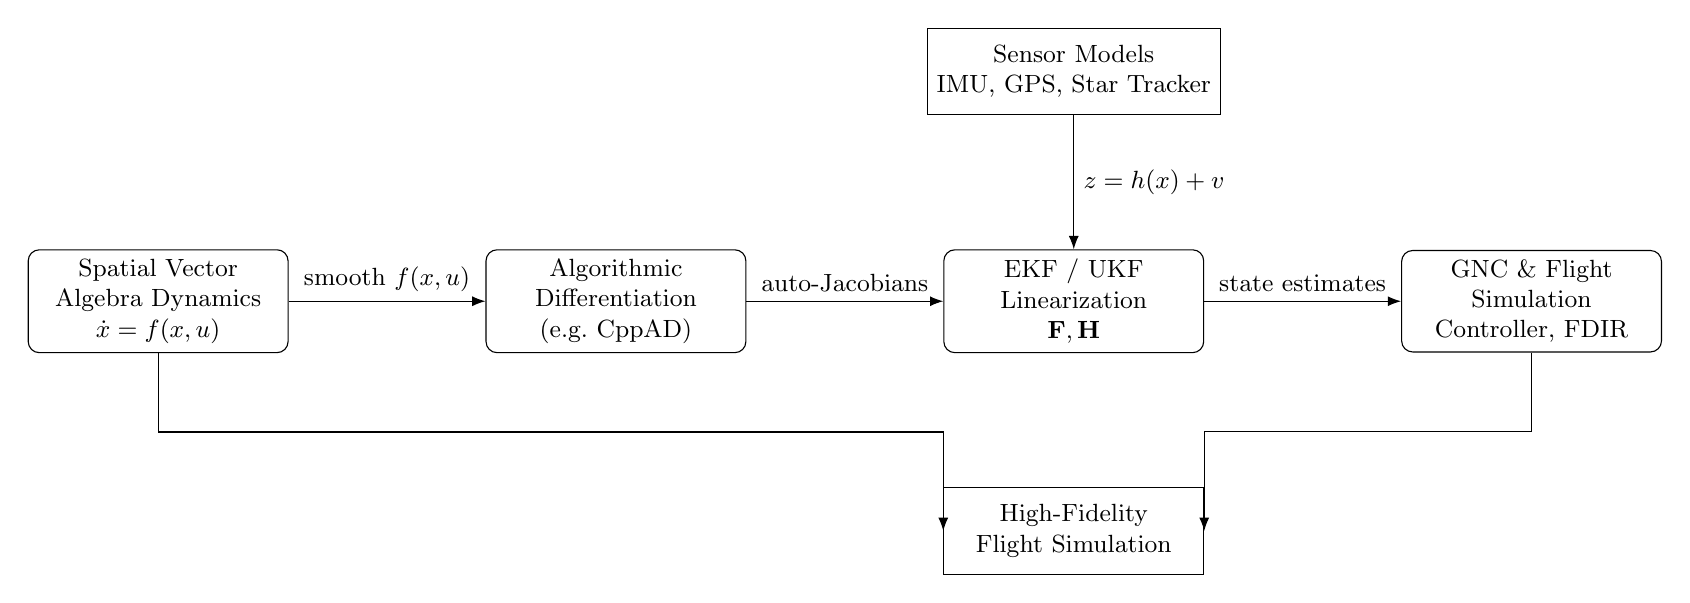
\begin{tikzpicture}[
  node distance = 2.5cm,
  >=Latex,
  process/.style = {rectangle, rounded corners, draw, align=center,
                    minimum width=3.3cm, minimum height=1.1cm},
  data/.style    = {rectangle, draw, align=center,
                    minimum width=3.3cm, minimum height=1.1cm},
  every node/.style = {font=\small}
]

% Nodes
\node[process] (sva) {Spatial Vector\\Algebra Dynamics\\$\dot{x} = f(x,u)$};
\node[process, right=of sva] (ad) {Algorithmic\\Differentiation\\(e.g.\ CppAD)};
\node[process, right=of ad] (ekf) {EKF / UKF\\Linearization\\$\mathbf{F}, \mathbf{H}$};
\node[process, right=of ekf] (gnc) {GNC \& Flight\\Simulation\\Controller, FDIR};

\node[data, above=1.7cm of ekf] (sensors) {Sensor Models\\IMU, GPS, Star Tracker};

\node[data, below=1.7cm of ekf] (sim) {High-Fidelity\\Flight Simulation};

% Main pipeline arrows
\draw[->] (sva) -- node[above]{smooth $f(x,u)$} (ad);
\draw[->] (ad) -- node[above]{auto-Jacobians} (ekf);
\draw[->] (ekf) -- node[above]{state estimates} (gnc);

% Sensors to EKF
\draw[->] (sensors.south) -- node[right]{$z = h(x) + v$} (ekf.north);

% Simulation connections
\draw[->] (sva.south) -- ++(0,-1) -| (sim.west);
\draw[->] (gnc.south) -- ++(0,-1) -| (sim.east);

\end{tikzpicture}
\end{document}
